\documentclass[10pt]{article}

\usepackage[english]{babel}
\usepackage[latin1]{inputenc}
\usepackage[T1]{fontenc}
\usepackage{graphicx}
\usepackage{geometry}
\usepackage{amsmath,amssymb}
\usepackage{color}
\usepackage{bm}
\usepackage{epstopdf}
\usepackage{dsfont}
\usepackage{tikz}


\DeclareMathOperator*{\argmin}{argmin}
\DeclareMathOperator*{\argmax}{argmax}

\newcommand{\rr}{\mathbb{R}}
\newcommand{\zz}{\mathbb{Z}}
\newcommand{\indep}{\ensuremath{\,\bot\!\!\!\bot\,}} %% The symbol for independent

\begin{document}


\begin{center}
\huge\textbf{Probabilistic Graphical Model\\ \Large
Assignment 1}\normalsize \\
\vspace{0.5cm}
Vincent BODIN \& Thomas MOREAU
\end{center}

\hrulefill
\vspace{1cm}


\section{Distributions factorizing in a graph}


\textbf{(a) }\begin{itemize}
\item We want to show that if $i \rightarrow j$ is a covered edge, then we can reverse it without affecting the factorizing property. Without loss of generality we can always assume that the graph is like the one shown in Fig.(\ref{fig1}). Indeed it suffices to write that we want to have:
\begin{equation}
\begin{array}{r l l}
p(x) \in \mathcal{L}(G) 	& \iff & \displaystyle p(x) = \left( \prod_{p\in \{1,\cdots, n\} - \{i,j\} } p(x_p | x_{\pi_p}) \right) p(x_i | x_{\pi_i}) p(x_j | x_i, x_{\pi_i}) \\ 
p(x) \in \mathcal{L}(G')  & \iff & \displaystyle p(x) = \left( \prod_{p\in \{1,\cdots, n\} - \{i,j\} } p(x_p | x_{\pi_p}) \right) p(x_j | x_{\pi_i}) p(x_i | x_j, x_{\pi_i})
\end{array}
\end{equation}
Hence this implies that we can forget about all the other terms than the one represented in Fig.(\ref{fig1}).
\begin{figure}[h!]
\centering
\begin{tikzpicture}
	[scale=.8]
	\node (n1) at (1,1) {$\pi_i$};
	\node (n2) at (3,3)  {i};
	\node (n3) at (5,1) {j};
	\foreach \from/\to in {n1/n2,n2/n3,n1/n3}
	\draw[->] (\from) -- (\to);
\end{tikzpicture}
\caption{Graph with covered edge}
\label{fig1}
\end{figure}

We denote $p_{\pi_i}(x)$ the probability given $x_{\pi_i}$. As this is a probability, we can apply to it the so-called Bayes formula: 
\begin{equation}
p_{\pi_i}(x_i) p_{\pi_i}(x_j | x_i) = p_{\pi_i}(x_j) p_{\pi_i}(x_i | x_j) 
\label{eq:}
\end{equation}
proving that $\mathcal{L}(G) = \mathcal{L}(G')$.


\item We need to show that in the case of a tree there is equivalence between: $X_i \indep X_{\text{nd}(i)} | X_{\pi(i)}$ and $X_A \indep X_B | X_C$ if $A$ and $B$ are separated by $C$. It is pretty straightforward as we notice that that d-separation is equivalent to separation in this kind of graph because there is no V-structure. Hence we can deduce from this the series of equivalence:
\begin{equation}
p(x)\in\mathcal{L}(G) \Leftrightarrow X_i \indep X_{\text{nd}(i)} | X_{\pi(i)} \Leftrightarrow X_A \indep X_B | X_C \Leftrightarrow \mathcal{L}(G')
\end{equation}



\end{itemize}


\textbf{(b)} We assume we have an undirected graph $G = (V,E)$.
\begin{itemize}
\item Assume $|V| = 1$ then it is obvious that $G' = (V,\emptyset)$ will verify $\mathcal{L}(G) = \mathcal{L}(G')$.

\item Assume $|V| = 2$. If we assume $G$ is not connected, then we get two graphs of size $1$ for which we have already seen it was not possible. From now on, we will only consider connected graphs. Then the result is once again obvious because we obtain a complete graph for which we know it does not work. That is a new indication, we have to take a connected graph non complete from now on. 

\item Assume $|V| = 3$, then as we cannot deal with complete graph, we only have two edges. Take a Markov chain or latent cause model, we know by the question (a) that both of them will give the same factorization as in $G$. Hence we have to look farther.

\item Assume $|V| = 4$, we have to put at least three edges to get a connected graph but in this case taking $G'$ a Markov chain with the same edges as in $G$ would lead to $\mathcal{L}(G) = \mathcal{L}(G')$. Hence we have to put four edges. Let us take the following graph as in Fig.(\ref{fig4}).
\begin{figure}[h!]
\centering
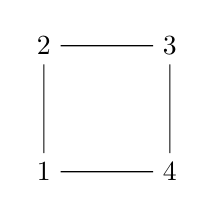
\begin{tikzpicture}
	[scale=.8]
	\node (n1) at (1,1) {1};
	\node (n2) at (1,3) {2};
	\node (n3) at (3,3) {3};
	\node (n4) at (3,1) {4};
	\foreach \from/\to in {n1/n2,n2/n3,n3/n4,n4/n1}
	\draw (\from) -- (\to);
\end{tikzpicture}
\caption{Graph such that there no $G'$ directed that verifies $\mathcal{L}(G) = \mathcal{L}(G')$}
\label{fig4}
\end{figure}

Let us prove there is no directed graph $G'$ such that $\mathcal{L}(G) = \mathcal{L}(G')$. In order to have $\mathcal{L}(G') = \mathcal{L}(G)$, $G'$ need to have the same number of vertices. It also needs to be connected as $G$ is connected (else it would imply by taking the connected components that a smaller set of $G'$ would also work which we excluded). 

Let us prove that the DAG associated has exactly four edges as well. The only way to have a different number of edges is that the DAG has a V-structure and then the moralized gets one new edge. From this remark we can infer that there can only be less edges in the DAG than in the undirected graph. Having one and two edges automatically lead to a non connected graph which is prohibited. Taking only three edges implies that we have a kind of C in the graph, for instance $(1,2)$, $(2,3)$, $(3,4)$ could be the edges. But in this case if we want the undirected graph related to have four edges, we need it to have a V-structure, which will necessarily be in a node that has two neighbors. Hence it cannot lead to a graph like the one in Fig.(\ref{fig4}) - it leads to a graph composed of a triangle plus a node linked with only one edge to this triangle.

As we need a DAG also, it implies that $G'$ will at least have a V-structure and look like Fig.(\ref{fig5}).
\begin{figure}[h!]
\centering
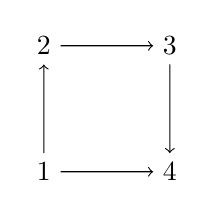
\begin{tikzpicture}
	[scale=.8]
	\node (n1) at (1,1) {1};
	\node (n2) at (1,3) {2};
	\node (n3) at (3,3) {3};
	\node (n4) at (3,1) {4};
	\foreach \from/\to in {n1/n2,n2/n3,n3/n4,n1/n4}
	\draw[->] (\from) -- (\to);
\end{tikzpicture}
\caption{Graph such that there no $G'$ directed that verifies $\mathcal{L}(G) = \mathcal{L}(G')$}
\label{fig5}
\end{figure}

What is important is that there is a V-structure in, say node 4, as in the previous figure. Then factorizing in $G'$ introduces a $p(x_4| x_1,x_3)$ which is not a clique in $G$.

\end{itemize}



\section{d-separation}

\textbf{(a) }$S$ separates $A$ and $B$ in $G_M$ which implies that for every chain $c(a,b)$ from $a\in A$ to $b\in B$, there exists $s\in S$ such that $d\in c(a,b)$. To facilitate the drawings we just assume the chain is $(a,s,b)$. We have two possibilities shown in Fig.(\ref{fig6}), either we have no V-structure or we have one.
\begin{figure}[h!]
\centering
\begin{tikzpicture}
	[scale=.8]
	\node (n1) at (1,1) {$a$};
	\node (n2) at (3,3) {$s$};
	\node (n3) at (5,1) {$b$};
	\foreach \from/\to in {n1/n2,n2/n3}
	\draw[->] (\from) -- (\to);
	
	\node (n4) at (7,1) {$a$};
	\node (n5) at (9,3) {$s$};
	\node (n6) at (11,1) {$b$};
	\foreach \from/\to in {n4/n5,n6/n5}
	\draw[->] (\from) -- (\to);
	\foreach \from/\to in {n4/n6}
	\draw[red] (\from) -- (\to);
\end{tikzpicture}
\caption{(left) generic case with no V-structure; (right) V-structure}
\label{fig6}
\end{figure}

If we do not have any V-structure then we are directly blocked by $s\in S$. Assume now we have a V-structure in $s$, that would imply that an edge - drawn in red - was in $G_M$ which contradicts the fact that $S$ separated $A$ and $B$ in $G_M$. Hence there cannot be any V-structure and then $A$ and $B$ are separated by $S$ in $G$.\\



\textbf{(b) }We give a counter example in Fig.(\ref{7}). 
\begin{figure}[h!]
\centering
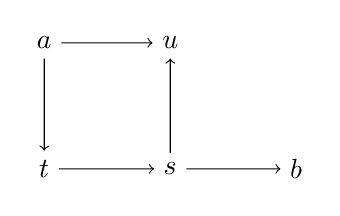
\begin{tikzpicture}
	[scale=.8]
	\node (n1) at (1,1) {$t$};
	\node (n2) at (1,3) {$a$};
	\node (n3) at (3,3) {$u$};
	\node (n4) at (3,1) {$s$};
	\node (n5) at (5,1) {$b$};
	\foreach \from/\to in {n2/n1,n1/n4,n2/n3,n4/n3,n4/n5}
	\draw[->] (\from) -- (\to);
\end{tikzpicture}
\caption{Counter-example}
\label{fig7}
\end{figure}
We set $A=\{a\}, B=\{b\}, S=\{s\}$ and $T=\{t\}$. Then $A$ and $B$ are d-separated by $S$ because every chain that goes from $A$ to $B$ passes through $s$ and there is no V-structure. $A$ and $S$ are d-separated by $T$ because a chain going from $A$ to $S$ passes either through $t$ that is not a V-structure or through $u$ that is one but who have no descendant in $T$. But $A$ and $B$ are not d-separated by $T$ since a chain can go from $A$ to $B$ through $(a,u,s,b)$ and $(a,u,s)$ is a V-structure but $t$ is a descendant of $s$.\\





\textbf{(c) }
\begin{itemize}
\item $X_{\{1,2\}} \indep X_4 |\ X_3$ is true. A chain from $A$ to $B$ passes through $(a,8,b)$ that is a V-structure with no descendant in $\{3\}$.

\item $X_{\{1,2\}} \indep X_4 |\ X_5$ is false. A chain from $A$ to $B$ passes through $(a,8,b)$ that is a V-structure and $\{5\}$ is a descendant of 8.

\item $X_1 \indep X_6 |\ X_{\{ 2,4,7 \}}$ is true. A chain from $A$ to $B$ passes through $(8,7,6)$ without a V-structure.
\end{itemize}



Thus, we have $p(x) \in \mathcal{L}(G')$. By symmetry, we have $\mathcal{L}(G) = \mathcal{L}(G')$.


\section{Implementation - Gaussian mixtures\\}

\emph{(a)}

\begin{figure}
\begin{tabular}{c c}
\includegraphics[width=7cm]{../figures/Kmeans_train.eps}
\includegraphics[width=7cm]{../figures/Kmeans_test.eps}
\end{tabular}
\end{figure}
\end{document}
